The question refers to ``the same sentiment classification problem in (g)''. We read this as the hotel-review project of (h): the reviews now come with rating scores, but some of those scores are wrong.
Training labels derived from the ratings are therefore \emph{noisy}.

\subsection*{How our classifier would be affected}

\paragraph{Sources and types of noise.}
Rating errors on review sites are rarely uniform~\cite{song2023learning}. Three kinds can be distinguished:
\begin{itemize}
  \item \emph{Random errors}, such as mis-clicks or swapped scales, are roughly \emph{symmetric}.
  \item \emph{Systematic errors} are \emph{class-conditional}. A guest may write a positive text but give a low score because of the price or a single incident, or a hotel may receive inflated scores. Noise then runs mainly in one direction.
  \item \emph{Instance-dependent errors} concentrate on ambiguous, mixed or sarcastic reviews, which are exactly the hard cases.
\end{itemize}

\paragraph{Effect on training.}
A discriminative classifier fits the labels it is given.
Over-parameterised neural networks can memorise even completely random labels. They do tend to learn the clean, dominant patterns first and only later fit the noise.
So a fine-tuned RoBERTa or a BiLSTM trained to convergence on noisy ratings would gradually absorb the errors, and its decision boundary and confidence estimates would suffer. Early stopping on clean data delays this but does not prevent it.
A regularised linear TF-IDF model cannot memorise as freely, but its weights are biased in the same way.
Class imbalance amplifies the damage. With an 85:15 class ratio, flipping each label independently with probability 20\% means only 41\% of the reviews labelled ``negative'' are truly negative, because flipped positives outnumber the real negatives.
The minority class, usually the one that matters most to a hotel, is affected first.

\paragraph{Effect on evaluation.}
If the validation and test labels are noisy too, measured accuracy underestimates the true accuracy, and model selection and threshold tuning chase the noise.
A small, manually verified clean set is therefore essential for any of the remedies below.

\subsection*{Experiment: injecting label noise into our data}
To quantify these effects we corrupted the labels of our 5{,}909 training-part reviews and kept the 1{,}492-review validation split clean.
We used two noise models:
\begin{itemize}
  \item \emph{symmetric}: every label is flipped with probability 0, 5, 10 or 20\%;
  \item \emph{positive$\to$negative}: only positive labels are flipped, with probability 5, 10 or 20\%, mimicking a positive text given a low score.
\end{itemize}
The base model is TF-IDF (word 1--2-grams) + LR, and each setting is repeated with 3 seeds.
Methods M1--M3 rely on 5-fold out-of-fold probabilities $p(x)$ computed on the noisy training part, with the same grouped folds as in (b). We compared four strategies:
\begin{itemize}
  \item \textbf{M0, baseline}: train on the noisy labels.
  \item \textbf{M1, sample selection (Confident Learning)}~\cite{northcutt2021confident}. For each class $j$, set the threshold $t_j$ to the mean predicted probability of $j$ over samples labelled $j$. A sample is flagged when its most probable class among those with $p_k \ge t_k$ differs from its given label. Flagged samples are removed and the model is retrained.
  \item \textbf{M2, label correction}: a label is flipped when the out-of-fold model assigns more than 0.9 probability to the opposite class.
  \item \textbf{M3, re-weighting}: each sample is weighted by the out-of-fold probability of its given label.
\end{itemize}

\begin{table}[t]
\centering
\caption{Validation results under injected label noise (mean $\pm$ std over 3 seeds). Left block: Macro-F1 at threshold~0.5. Right block: ROC-AUC, which does not depend on the threshold. ``Neg.\ prec.'' is the fraction of training reviews labelled negative that are truly negative. Without class weights and threshold tuning, the clean baseline's Macro-F1 (0.789) is lower than the tuned TF-IDF model in (g) (0.851).}
\label{tab:i-noise}
\small
\setlength{\tabcolsep}{3.5pt}
\begin{tabular}{l r c cccc cccc}
\toprule
 & & Neg. & \multicolumn{4}{c}{Macro-F1 @ 0.5} & \multicolumn{4}{c}{ROC-AUC} \\
\cmidrule(lr){4-7}\cmidrule(lr){8-11}
Noise & Rate & prec. & M0 & M1 & M2 & M3 & M0 & M1 & M2 & M3 \\
\midrule
--          & 0\%  & 1.00 & .789 & \textbf{.810} & .765 & .692 & \textbf{.950} & .948 & .946 & .945 \\
Symmetric   & 5\%  & 0.77 & .789 & \textbf{.814} & .789 & .698 & .938 & \textbf{.944} & \textbf{.944} & \textbf{.944} \\
            & 10\% & 0.60 & .772 & \textbf{.805} & .765 & .690 & .910 & .936 & .929 & \textbf{.939} \\
            & 20\% & 0.41 & .720 & \textbf{.792} & .754 & .724 & .837 & \textbf{.909} & .878 & .907 \\
Pos$\to$neg & 5\%  & 0.77 & .802 & \textbf{.823} & .812 & .728 & .935 & \textbf{.944} & \textbf{.944} & \textbf{.944} \\
            & 10\% & 0.63 & .806 & \textbf{.819} & .809 & .769 & .917 & .940 & .936 & \textbf{.941} \\
            & 20\% & 0.46 & .778 & \textbf{.819} & .796 & .814 & .901 & .931 & .917 & \textbf{.933} \\
\bottomrule
\end{tabular}\\[2pt]
\footnotesize Standard deviations are 0.003--0.020 for Macro-F1 and below 0.008 for AUC; full values are in \texttt{outputs/noise\_exp/summary.csv}.
\end{table}

\begin{figure}[t]
\centering
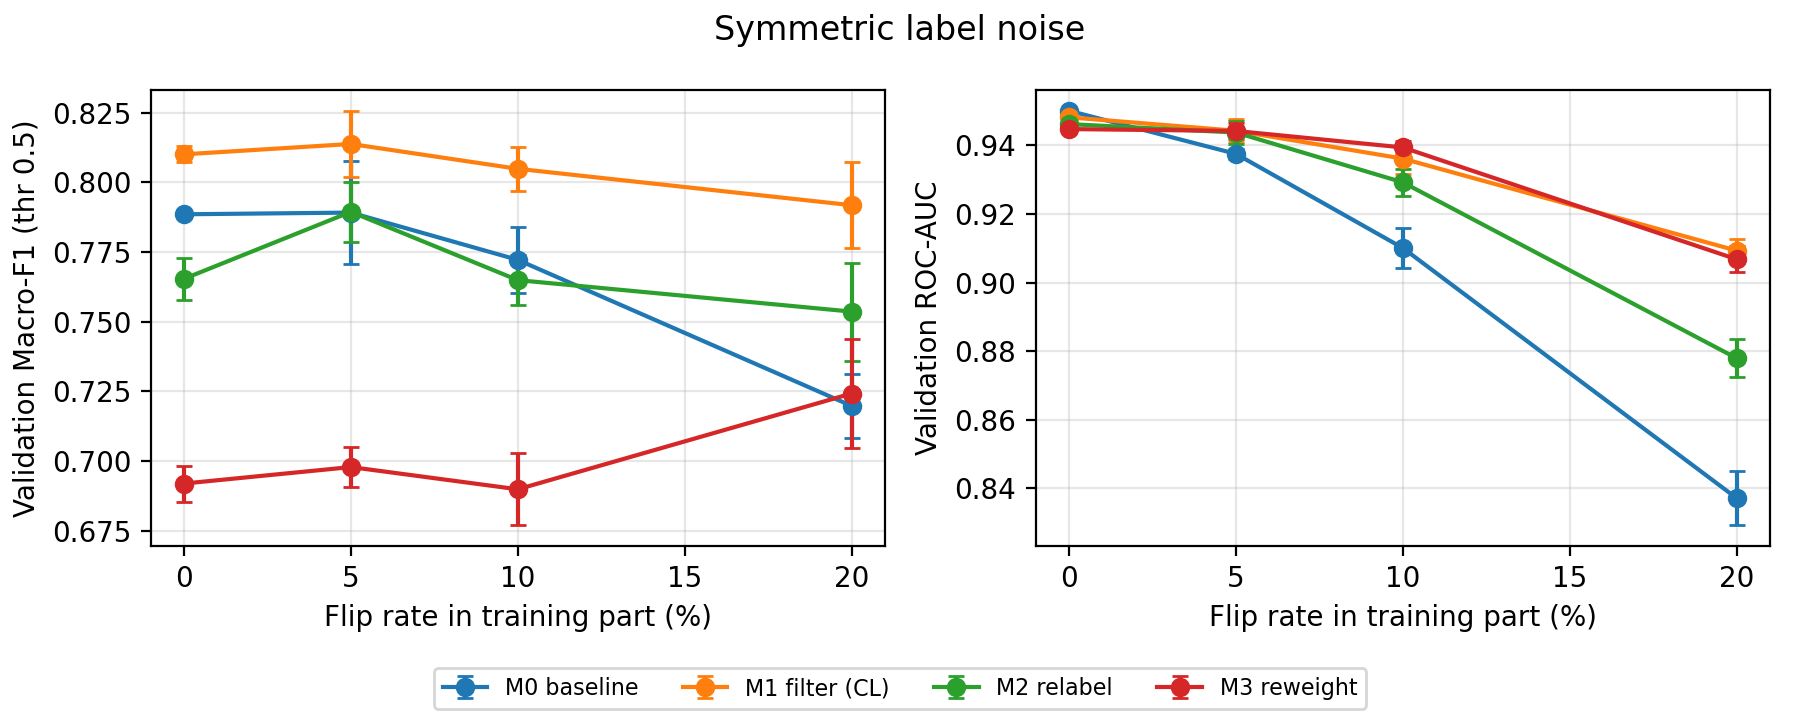
\includegraphics[width=\textwidth]{noise_symmetric.png}\\[4pt]
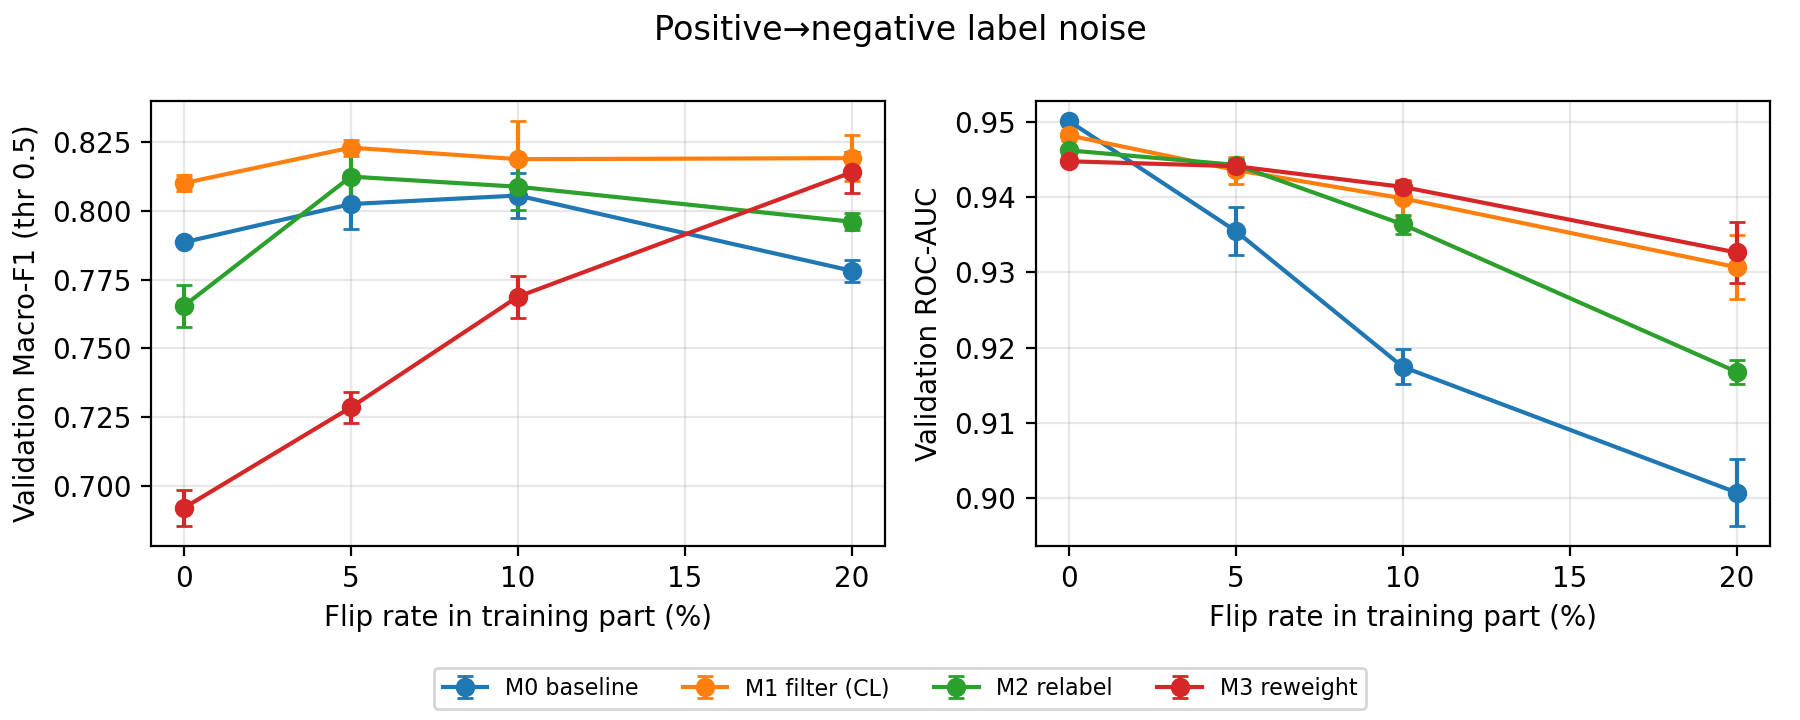
\includegraphics[width=\textwidth]{noise_pos2neg.png}
\caption{Validation Macro-F1 at threshold 0.5 (left) and ROC-AUC (right) as the training-label flip rate grows. Error bars show $\pm1$ std over 3 seeds.}
\label{fig:i-noise}
\end{figure}

\paragraph{Findings.}
Table~\ref{tab:i-noise} and Figure~\ref{fig:i-noise} lead to five observations.
\begin{enumerate}
  \item \textbf{Noise hurts, and imbalance makes it worse.} Under 20\% symmetric noise the baseline's AUC drops from 0.950 to 0.837, and its Macro-F1 from 0.789 to 0.720. The F1 of the negative class falls from 0.63 to 0.52.
  \item \textbf{Threshold-0.5 metrics can mislead.} Positive$\to$negative noise of 5--10\% slightly \emph{raises} the baseline's Macro-F1 at 0.5, although its AUC falls. The extra negative labels merely shift the decision boundary towards the minority class. This is why we also report AUC, and why thresholds must be tuned on clean data.
  \item \textbf{Sample selection (M1) is the most reliable method.} It gives the best Macro-F1 in every setting, and at 20\% symmetric noise it recovers AUC from 0.837 to 0.909. It removed 1{,}633 reviews on average; 44\% of them had actually been flipped, and it caught 61\% of all flipped labels. Even on the clean data it removed about 80 hard or ambiguous reviews and improved Macro-F1 by 0.02.
  \item \textbf{Label correction (M2) is precise but conservative.} 83--97\% of the labels it changed were truly wrong, but it changed only 200--280 of them, so its gains are moderate.
  \item \textbf{Re-weighting (M3) ranks well but needs re-calibration.} It matches M1 in AUC and is best under strong positive$\to$negative noise. However, its Macro-F1 at 0.5 is poor at low noise: negative reviews receive lower out-of-fold confidence, so re-weighting shrinks the minority class further. Combined with class weights or threshold tuning, this weakness would disappear.
\end{enumerate}
These results come from synthetic noise, a linear model and a single validation split. They show the size of the problem and the relative behaviour of the strategy families, not the gains to expect on real hotel ratings.

\subsection*{Three approaches to improve the algorithm}
The three families below follow the taxonomy of the recent survey by Song et al.~\cite{song2023learning}, where the individual methods named here are reviewed in detail.
\begin{enumerate}
  \item \textbf{Noise-robust losses and loss correction.} Replace plain cross-entropy with a loss that penalises confidently wrong labels less. Options include generalized cross-entropy, which interpolates between cross-entropy and the noise-tolerant MAE; symmetric cross-entropy; and label smoothing.
  When the noise is class-conditional, as with positive texts given low scores, one can instead estimate the $2\times2$ noise-transition matrix $T$ and correct the loss through it (forward/backward correction). $T$ can be estimated from a small clean subset.
  These methods change only the loss function of our RoBERTa fine-tuning, and add no extra cost.

  \item \textbf{Sample selection and data cleaning.} Exploit the fact that networks fit clean samples first, so small-loss samples are more likely to be correctly labelled.
  Co-teaching trains two networks and lets each one update on the small-loss samples chosen by the other. Confident Learning estimates the joint distribution of noisy and true labels from out-of-fold probabilities, then prunes or ranks the suspicious samples~\cite{northcutt2021confident}; this is our M1, the best method in our experiment.
  Flagged reviews can also be sent to annotators instead of being discarded.

  \item \textbf{Label correction and semi-supervised learning.} Instead of discarding suspicious samples, correct or down-weight them. Our M2 and M3 are simple versions.
  DivideMix fits a two-component mixture model to the per-sample losses to separate likely-clean from likely-noisy reviews. It then treats the noisy ones as \emph{unlabelled} data and trains on both parts with MixMatch-style semi-supervised learning.
  For hotel reviews, the text itself is a second, independent signal. A zero-shot model, for example our RoBERTa classifier or an LLM, can check each rating against its text, and the two can be combined into a corrected label.
\end{enumerate}

\paragraph{Recommended pipeline for the hotel project.}
\begin{enumerate}
  \item Manually verify a few hundred reviews to obtain a clean development set, and use it to estimate the noise rate and the transition matrix $T$.
  \item Fine-tune a pre-trained Transformer with a robust loss (GCE or label smoothing) and early stopping on the clean set.
  \item Run Confident Learning on out-of-fold predictions; relabel or drop the flagged reviews, sending the uncertain ones to annotators.
  \item Retrain, optionally with DivideMix-style semi-supervised learning on the doubtful part, and tune the decision threshold on the clean set.
\end{enumerate}
